\begin{table}[!p]
\vspace*{-\baselineskip}
\hspace*{-6mm}
\begin{tabular}{r@{}p{2.9cm}@{}p{2.9cm}@{}p{2.9cm}@{}p{2.9cm}@{}p{2.90cm}}
%\begin{tabular}{r@{}p{2.0cm}@{}p{2.0cm}@{}p{2.0cm}@{}p{2.0cm}@{}p{2.0cm}}
 & \textbf{~~~~~500} & \textbf{~~~~1000} & \textbf{~~~~2000} & \textbf{~~~~5000} & \textbf{~~~10000} \\
\textsc{mwst~} &
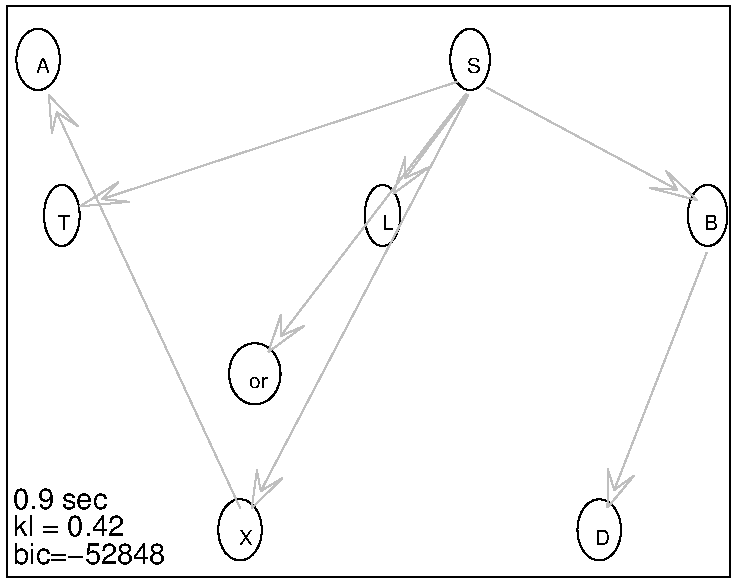
\includegraphics[width=29.34mm, height=26.7mm]{fig/MWST-ACA-500} &
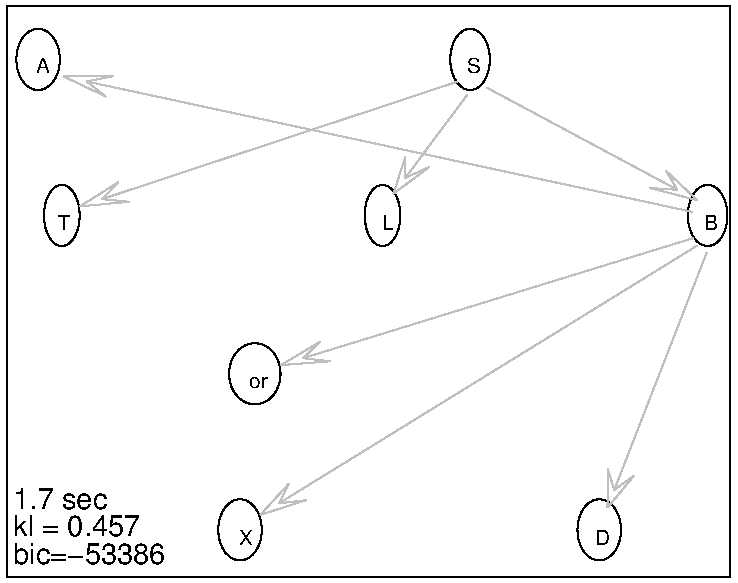
\includegraphics[width=29.34mm, height=26.7mm]{fig/MWST-ACA-1000} &
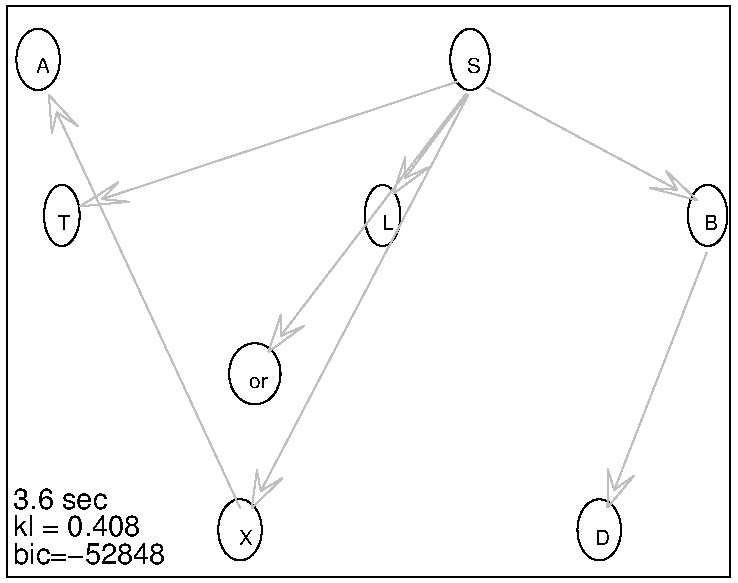
\includegraphics[width=29.34mm, height=26.7mm]{fig/MWST-ACA-2000} &
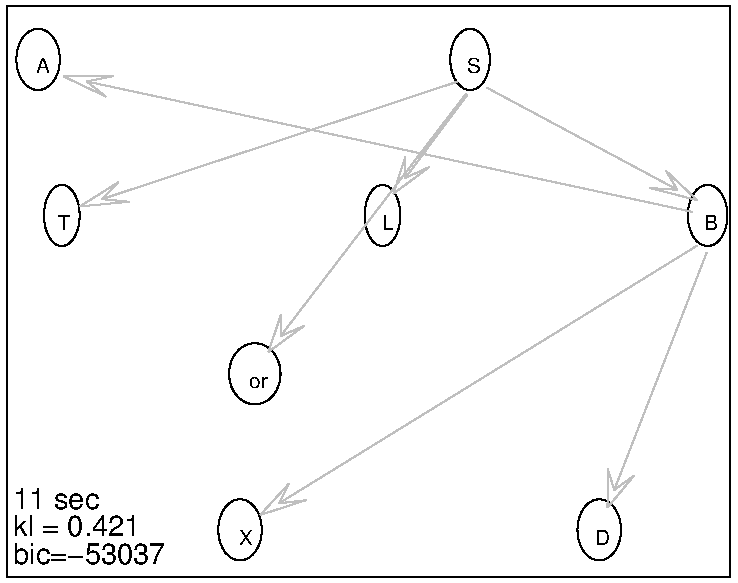
\includegraphics[width=29.34mm, height=26.7mm]{fig/MWST-ACA-5000} &
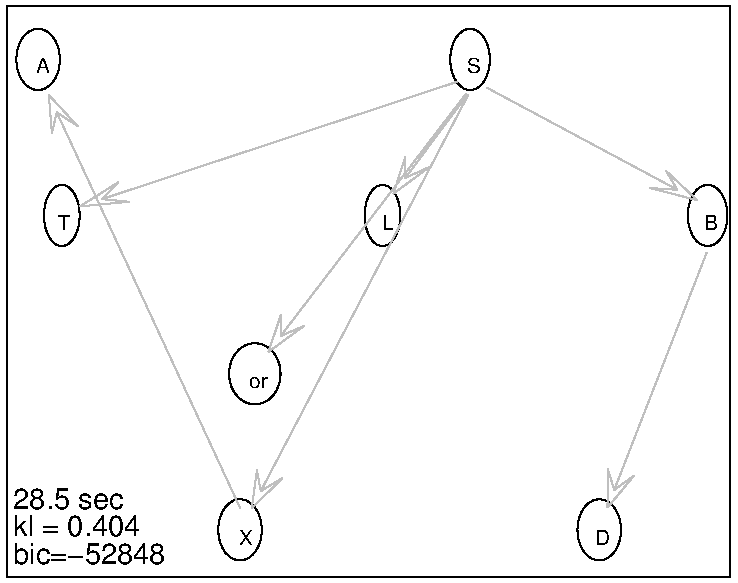
\includegraphics[width=29.34mm, height=26.7mm]{fig/MWST-ACA-10000} \\
\textsc{aca~}
& 9; -52848 & 9; -53386 & 9; -52848 & 9; -53037 & 9; -52848 \\
\textsc{mwst~} &
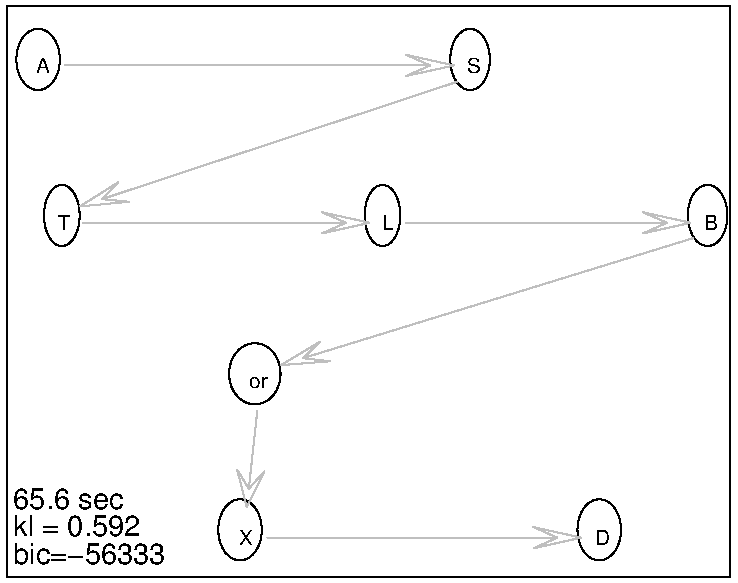
\includegraphics[width=29.34mm, height=26.7mm]{fig/MWST-EM-500} &
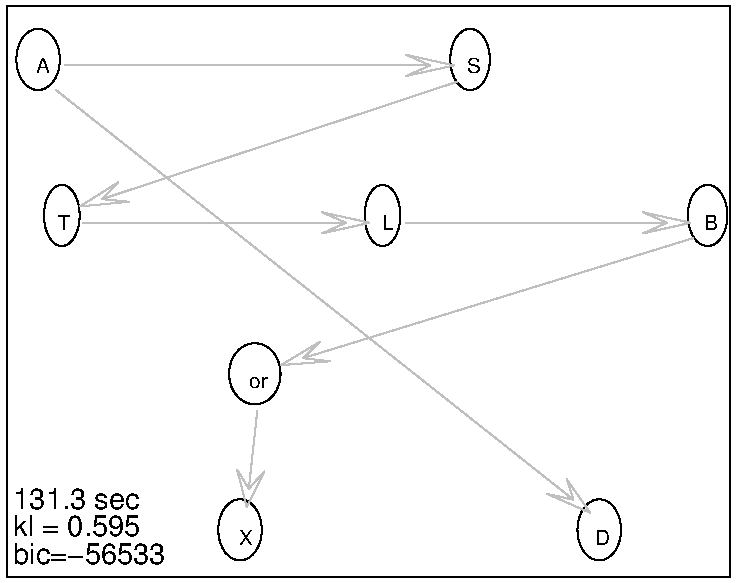
\includegraphics[width=29.34mm, height=26.7mm]{fig/MWST-EM-1000} &
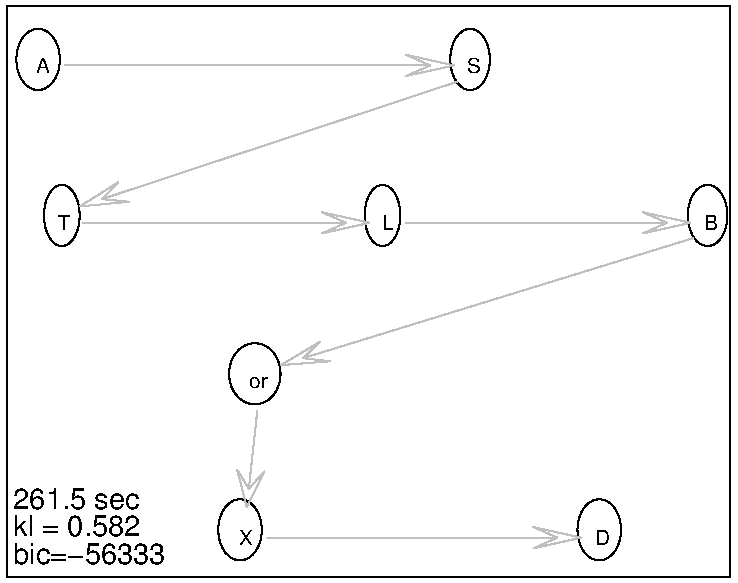
\includegraphics[width=29.34mm, height=26.7mm]{fig/MWST-EM-2000} &
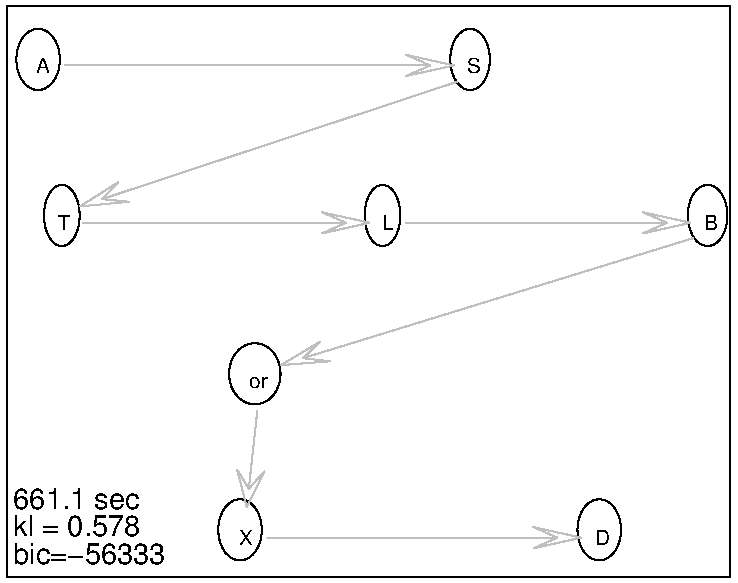
\includegraphics[width=29.34mm, height=26.7mm]{fig/MWST-EM-5000} &
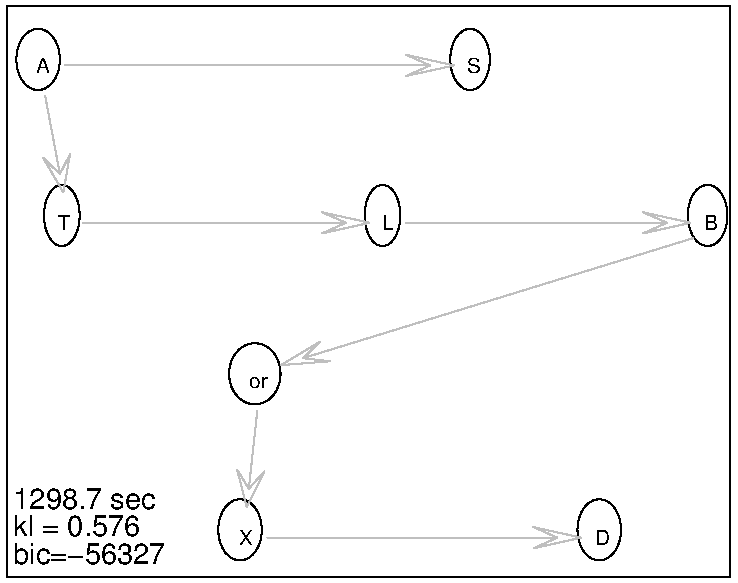
\includegraphics[width=29.34mm, height=26.7mm]{fig/MWST-EM-10000} \\
\textsc{em~}
& 13; -56333 & 13; -56533 & 13; -56333 & 13; -56333 & 11; -56327 \\
\textsc{gs~} &
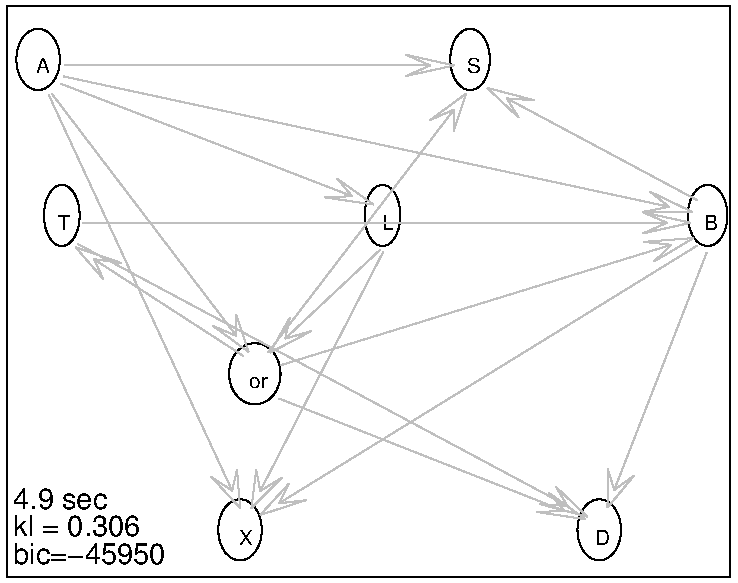
\includegraphics[width=29.34mm, height=26.7mm]{fig/GS-ACA-500} &
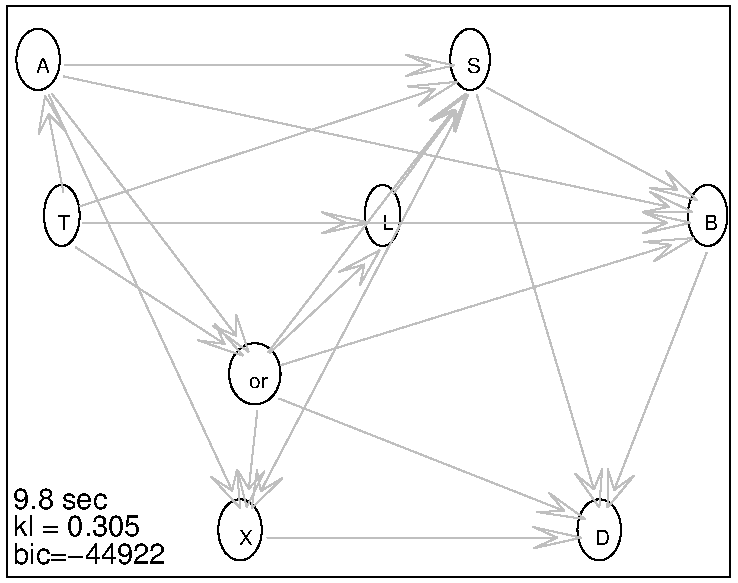
\includegraphics[width=29.34mm, height=26.7mm]{fig/GS-ACA-1000} &
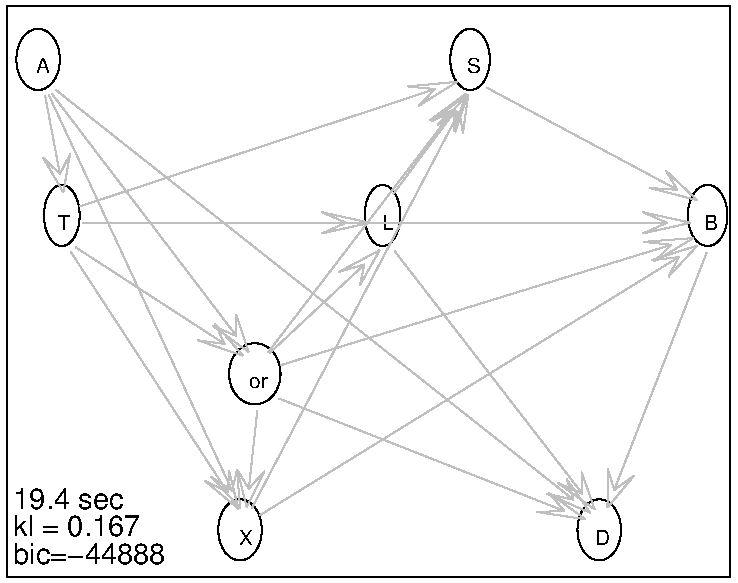
\includegraphics[width=29.34mm, height=26.7mm]{fig/GS-ACA-2000} &
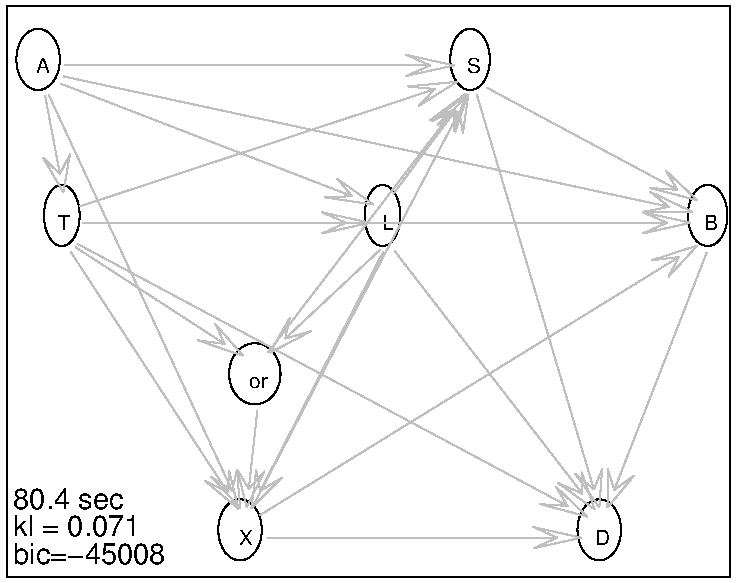
\includegraphics[width=29.34mm, height=26.7mm]{fig/GS-ACA-5000} &
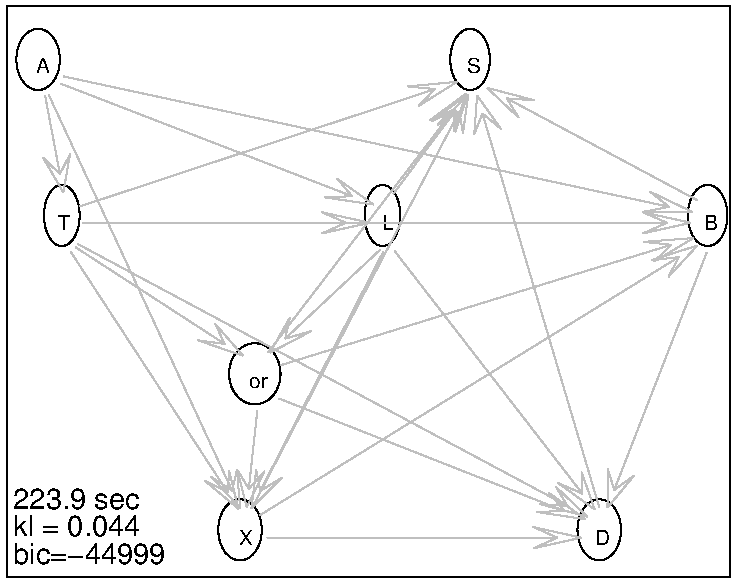
\includegraphics[width=29.34mm, height=26.7mm]{fig/GS-ACA-10000} \\
\textsc{aca~}
& 16; -45950 & 15; -44922 & 14; -44888 & 19; -45008 & 19; -44999 \\
\textsc{gs~} &
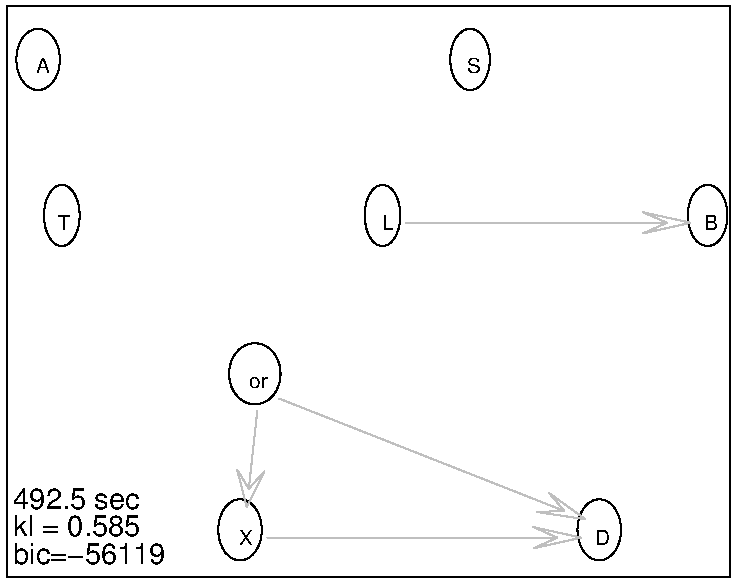
\includegraphics[width=29.34mm, height=26.7mm]{fig/GS-EM-500} &
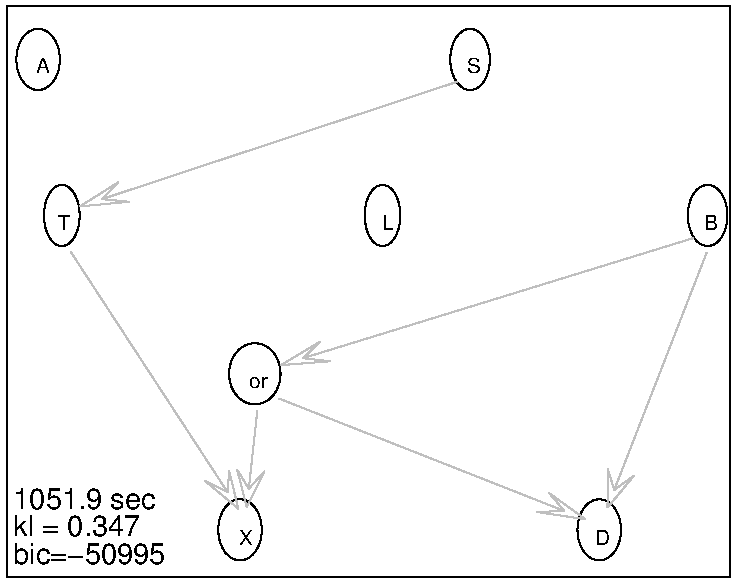
\includegraphics[width=29.34mm, height=26.7mm]{fig/GS-EM-1000} &
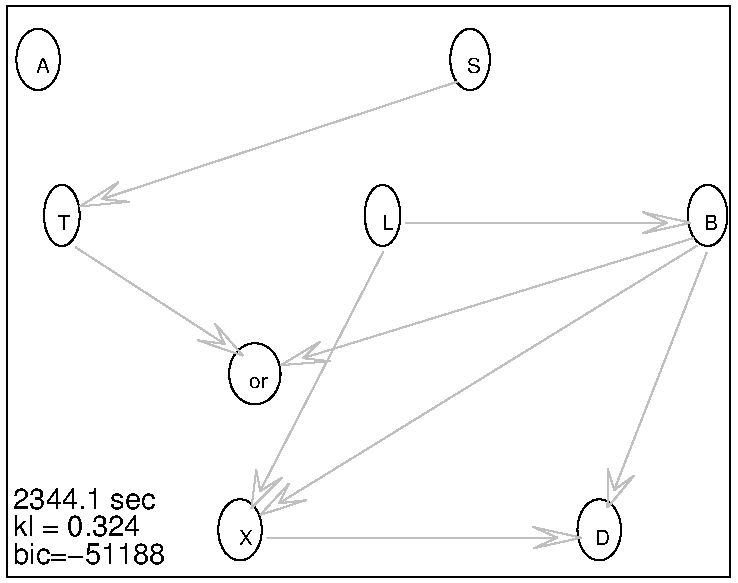
\includegraphics[width=29.34mm, height=26.7mm]{fig/GS-EM-2000} &
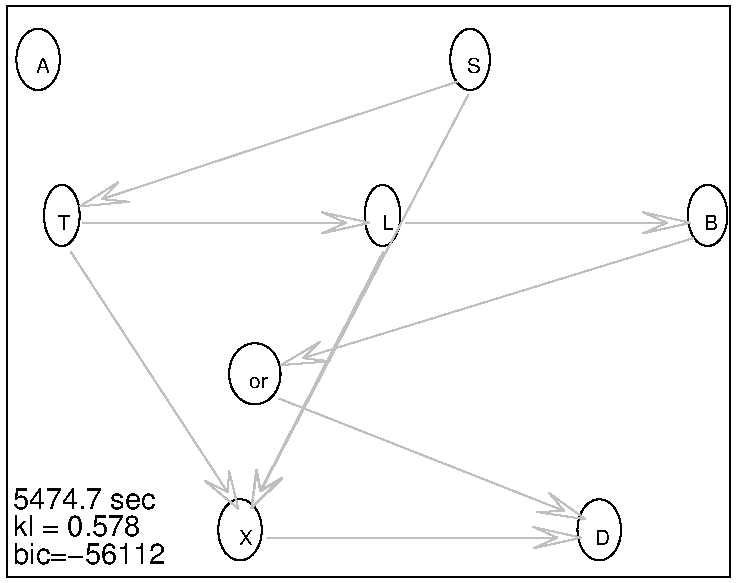
\includegraphics[width=29.34mm, height=26.7mm]{fig/GS-EM-5000} &
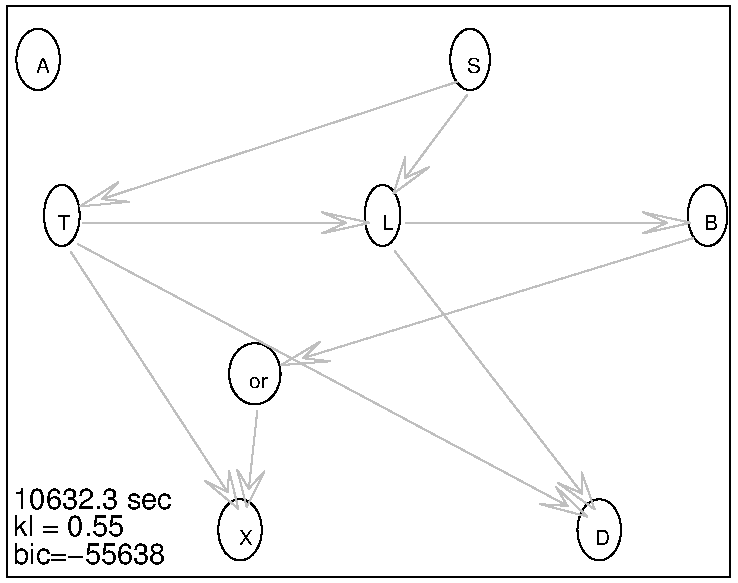
\includegraphics[width=29.34mm, height=26.7mm]{fig/GS-EM-10000} \\
\textsc{em~}
& 8; -56119 & 8; -50995 & 12; -51188 & 15; -56112 & 13; -55638 \\
\textsc{ges~} &
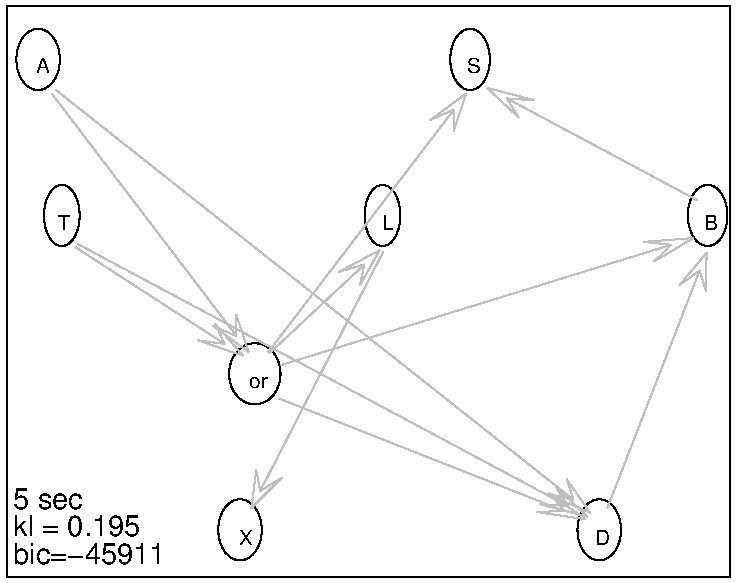
\includegraphics[width=29.34mm, height=26.7mm]{fig/GES-ACA-500} &
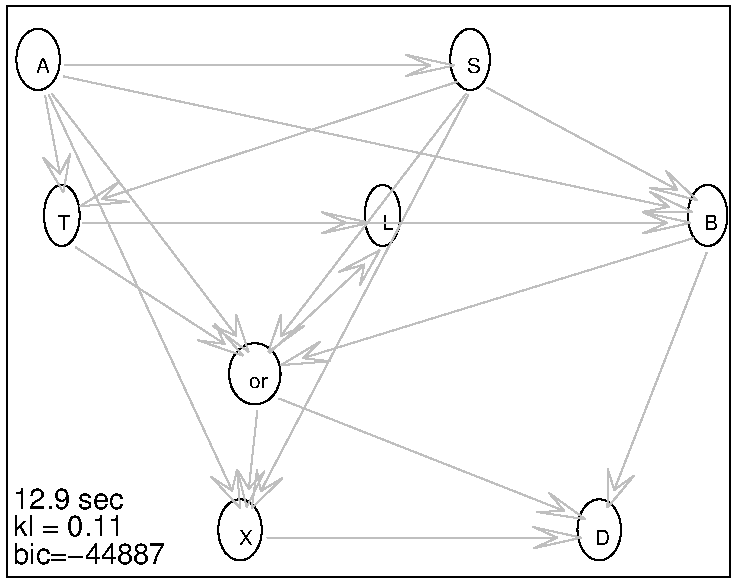
\includegraphics[width=29.34mm, height=26.7mm]{fig/GES-ACA-1000} &
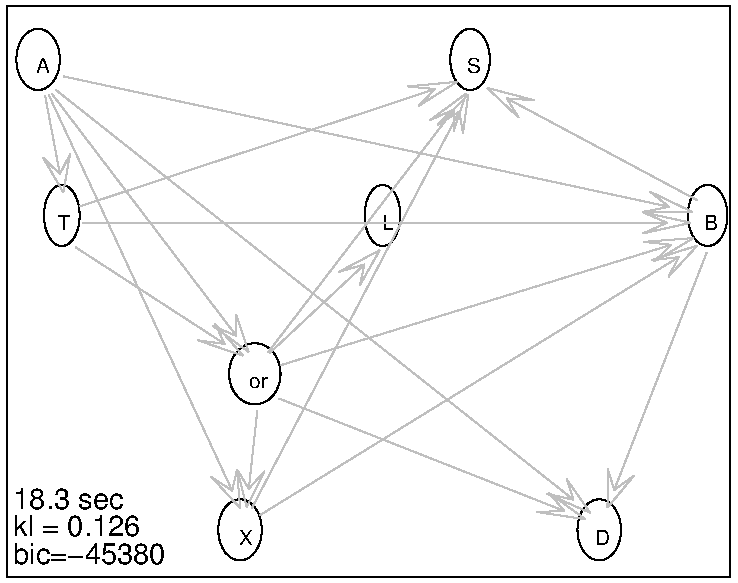
\includegraphics[width=29.34mm, height=26.7mm]{fig/GES-ACA-2000} &
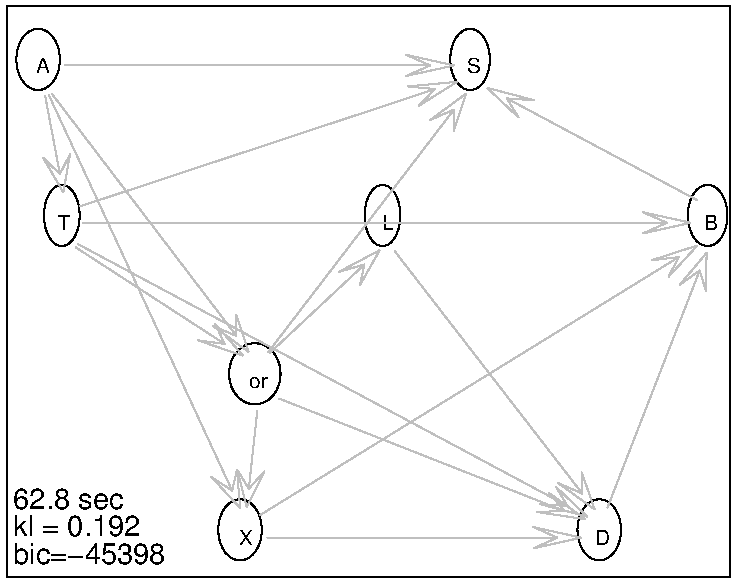
\includegraphics[width=29.34mm, height=26.7mm]{fig/GES-ACA-5000} &
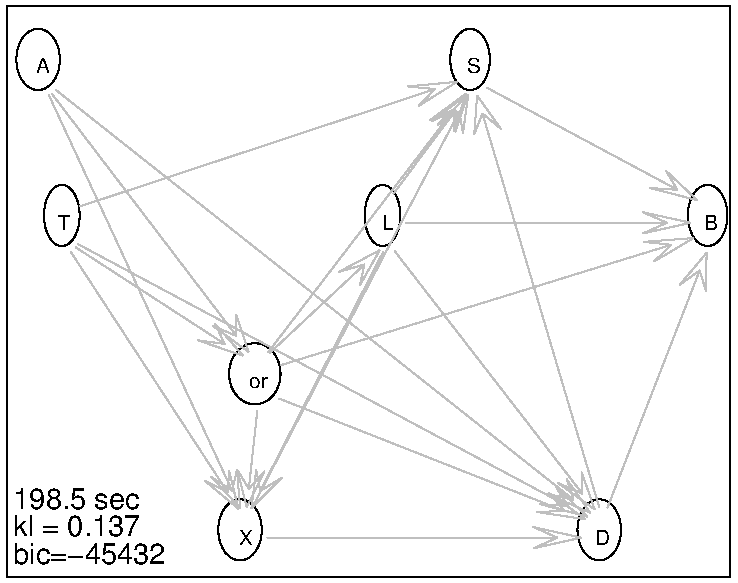
\includegraphics[width=29.34mm, height=26.7mm]{fig/GES-ACA-10000} \\
\textsc{aca~}
& 12; -45911 & 13; -44887 & 13; -45380 & 15; -45398 & 18; -45432 \\
\textsc{ges~} &
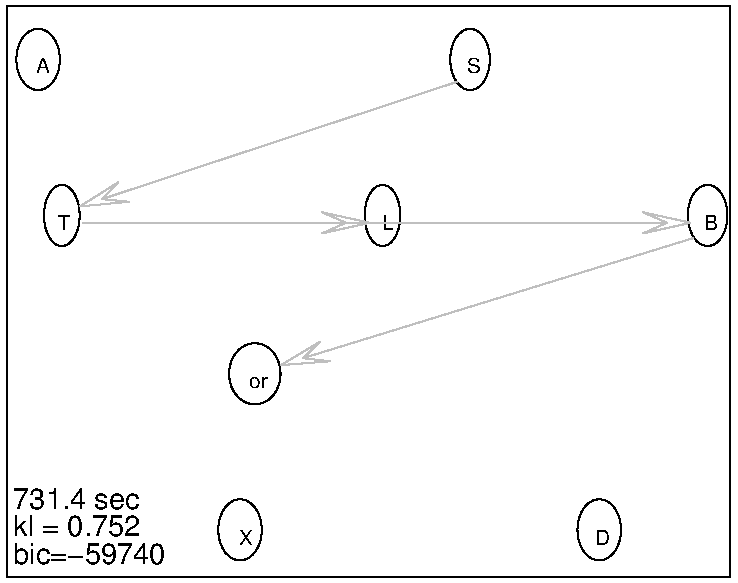
\includegraphics[width=29.34mm, height=26.7mm]{fig/GES-EM-500} &
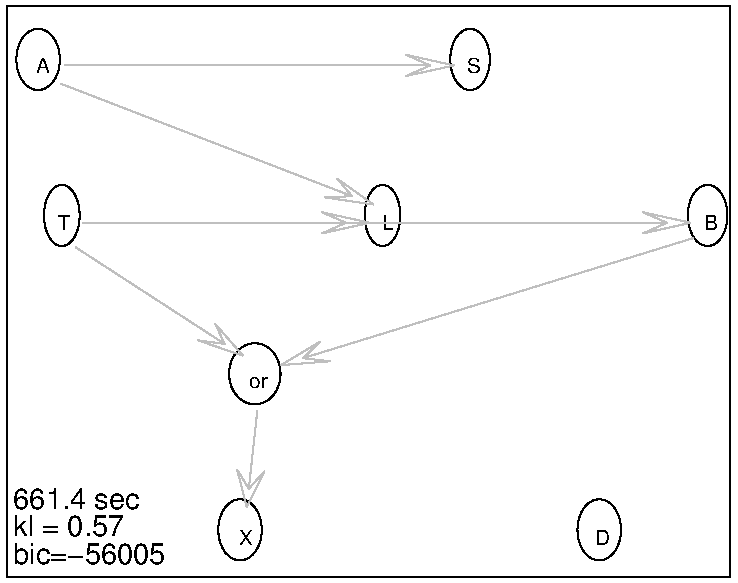
\includegraphics[width=29.34mm, height=26.7mm]{fig/GES-EM-1000} &
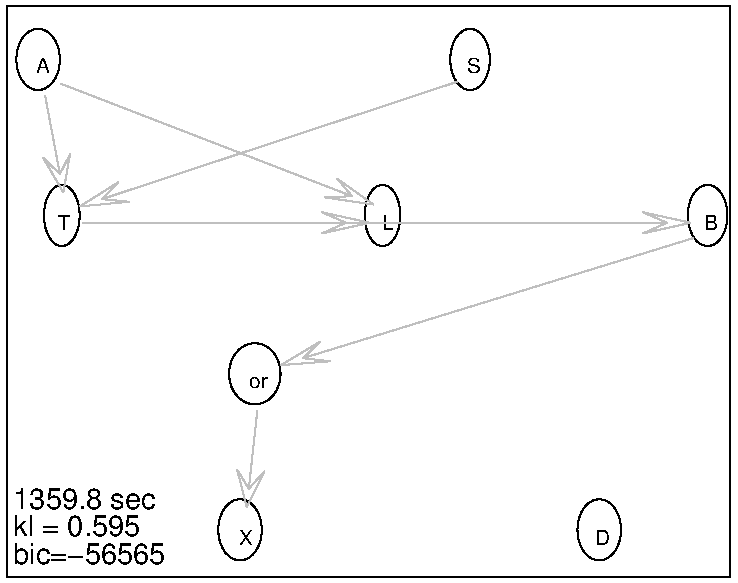
\includegraphics[width=29.34mm, height=26.7mm]{fig/GES-EM-2000} &
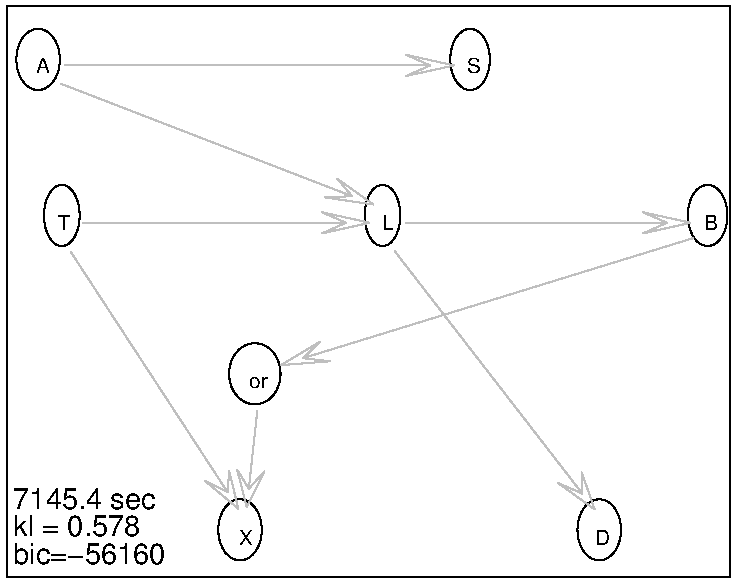
\includegraphics[width=29.34mm, height=26.7mm]{fig/GES-EM-5000} &
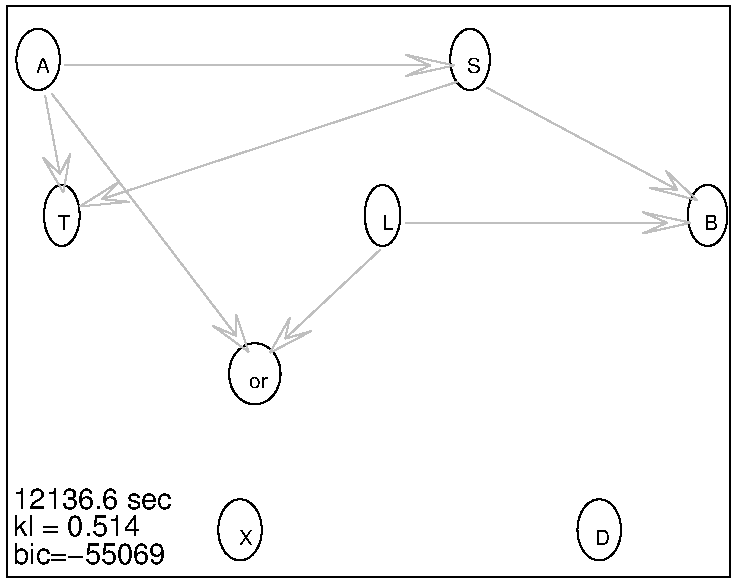
\includegraphics[width=29.34mm, height=26.7mm]{fig/GES-EM-10000} \\
\textsc{em~}
& 12; -59740 & 11; -56005 & 11; -56565 & 14; -56160 & 9; -55069 \\
\end{tabular}
\caption{Editing measures, networks and BIC scores obtained with different methods (in row) for several dataset lengths (in column). Computational time and Kullback-Leiber divergence means (on five parameters learning) are also printed in boxes.}
\label{inc1}
\end{table}
